%\documentclass[draft]{iseman}
\documentclass{iseman}


%%%   ページのマージン   %%%
% \evensidemargin 0.0in
% \oddsidemargin 0.0in
% \topmargin 0.0in
% \textwidth 6.5in
% \textheight 8.0in
% \headheight 0.0in
% \headsep 0.0in
% \footskip 0.0in

%%%   ページ数の設定   %%%
\setcounter{page}{1}

%%%   usepackage   %%%
\usepackage{graphicx}
\usepackage{amsfonts}
\usepackage{latexsym}
\usepackage{amssymb}
\usepackage{amsmath}
\usepackage{amsthm}
\usepackage{epsf}
\usepackage{bm}

%%% 追加パッケージ %%%
\usepackage{caption}

%%%   マクロ   %%%

% \def\b#1{\mbox{\boldmath ${#1}$}}

\renewcommand\figurename{図}
\renewcommand\tablename{表}
\renewcommand\refname{参考文献}

%\renewcommand\section{\@startsection {section}{1}{\z@}%
%                                   {3.5ex \@plus 1ex \@minus .2ex}%
 %                                  {1.3ex \@plus .5ex}%
  %                                 {\normalfont\small\bfseries\hspace{-2.5ex}\underline}}
%\renewcommand \thesection {\@arabic\c@section.\hspace{-1ex}}


\newcommand{\vzero}{\boldsymbol 0}
\newcommand{\vone}{\boldsymbol 1}
\newcommand{\va}{\boldsymbol a}
\newcommand{\vb}{\boldsymbol b}
\newcommand{\ve}{\boldsymbol e}
\newcommand{\vf}{\boldsymbol f}
\newcommand{\vg}{\boldsymbol g}
\newcommand{\vh}{\boldsymbol h}
\newcommand{\vn}{\boldsymbol n}
\newcommand{\vp}{\boldsymbol p}
\newcommand{\vu}{\boldsymbol u}
\newcommand{\vv}{\boldsymbol v}
\newcommand{\vx}{\boldsymbol x}
\newcommand{\vy}{\boldsymbol y}

\newcommand{\val}{\boldsymbol \alpha}
\newcommand{\vbe}{\boldsymbol \beta}
\newcommand{\vga}{\boldsymbol \gamma}
\newcommand{\vla}{\boldsymbol \lambda}
\newcommand{\vnu}{\boldsymbol \nu}
\newcommand{\vom}{\boldsymbol \omega}
\newcommand{\vth}{\boldsymbol \theta}
\newcommand{\vpi}{\boldsymbol \bm{\pi}}
\newcommand{\veta}{\boldsymbol \eta}
\newcommand{\vxi}{\boldsymbol \xi}

\newcommand{\MA}{\boldsymbol A}
\newcommand{\MB}{\boldsymbol B}
\newcommand{\MC}{\boldsymbol C}
\newcommand{\MD}{\boldsymbol D}
\newcommand{\ME}{\boldsymbol {\rm E}}
\newcommand{\MG}{\boldsymbol G}
\newcommand{\MH}{\boldsymbol H}
\newcommand{\MI}{\boldsymbol I}
\newcommand{\MK}{\boldsymbol K}
\newcommand{\MM}{\boldsymbol M}
\newcommand{\MO}{\boldsymbol O}
\newcommand{\MP}{\boldsymbol P}
\newcommand{\MQ}{\boldsymbol Q}
\newcommand{\MR}{\boldsymbol R}
\newcommand{\MS}{\boldsymbol S}
\newcommand{\MT}{\boldsymbol T}
\newcommand{\MV}{\boldsymbol V}
\newcommand{\MX}{\boldsymbol X}
\newcommand{\MLam}{\boldsymbol \Lambda}

\newcommand{\cA}{{\mathcal A}}
\newcommand{\cB}{{\mathcal B}}
\newcommand{\cC}{{\mathcal C}}
\newcommand{\cE}{{\mathcal S}^E}
\newcommand{\cG}{{\mathcal S}^G}
\newcommand{\cD}{{\mathcal D}}
\newcommand{\cP}{{\mathcal P}}
\newcommand{\cI}{{\mathcal I}}
\newcommand{\cL}{{\mathcal L}}
\newcommand{\cS}{{\mathcal S}}
\newcommand{\cT}{{\mathcal T}}
\newcommand{\cX}{{\mathcal X}}

\newcommand{\argmax}{\mathop{\rm arg~max}\limits}

\makeatother

%%%%%%%%%%%%%%%%%%%%%%%%%%%%%%%%%%%%%%%%%%%%%%%%%%%%%%%%%%%%%%%%%%%%%%%%%%%%%%%%%%%%%%%%%%%%%%%%%


\begin{document}

\noindent
\twocolumn[
	\begin{center}
	\Large{\bf マッチング制約のあるフレキシブルフローショップの性能評価に関する考察}
	\end{center}
	\vspace{\baselineskip}
	\begin{tabular}{@{}p{11zw}@{}p{11zw}@{}}
			\hfil
		{\small 広島大学工学部第二類}
		\hfil
		&
		\hfil
		{\small システム工学課程}
		\hfil
		\\
		\hfil
		{\small B132075}
		\hfil
		&
		\hfil
		{\small 森原~和也}
		\hfil
	\end{tabular}
	\begin{tabular}{@{}l@{}}
		{\small 指導教員: 岡村~寛之,土肥~正 } \\
		{\small 所  属: ディペンダブルシステム論研究室}
	\end{tabular}
	\vspace{2\baselineskip}
]


%%%%%%%%%%%%%%%%%%%%%%%%%%%%%%%%%%%%%%%%%%%%%%%%%%%%%%%%%%%%%%%%%%%%%%%%%%%%%%%%%%%%%%%%%%%%%%%%%%
\setcounter{page}{5}
\section{はじめに}\label{sec:intro}
製品の加工工程順に機械を配置し流れ作業を行うシステムをフローショップと呼び,その中でも各工程に複数の機械を配置し並列的に作業を行うシステムをフレキシブルフローショップ(FFS)と呼ぶ.FFSでは並列的な処理が行われるためシステム性能の評価が設計や計画において重要となる.Zhangら \cite{1} はマッチング処理制約を伴う4工程FFSについて,解析的な近似手法を用いてスループット及びジョブの系内滞在時間による性能評価を行った.本稿では文献 \cite{1} では考えられていなかったFFSにおける不良部品の発生が起こる4工程FFSについて,不良部品の発生を検知するための検査作業を行う工程数が2つであると仮定し,どの工程において検査を行うとスループットが最も高くなるのかを調べた.


\section{マッチング処理制約のある4工程FFS}
本稿では文献 \cite{1} と同様に4工程FFSを考える(図 \ref{fig:model}参照).第1工程では二種類の部品を別々のラインで加工して第2工程へ渡す.第2工程はマッチング工程と呼ばれ,前の工程から受け取った2つの部品を1度組み合わせて加工し,その後再び2つの部品に分解して次の工程に渡す.第3工程では第2工程で分解した2つの部品をそれぞれ別のラインで並列的に加工する.最後の第4工程は組み合わせ工程と呼ばれ,2つの部品を組み合わせてシステムを離脱させる.各工程には部品を配置するバッファがあり,次工程のバッファが埋まっている場合,前工程から部品を渡すことができないため前工程の処理が止まる.これをブロッキングと呼ぶ.またマッチング処理制約とは,第4工程で組み合わせる2つの部品は第2工程で処理されたペアでなければならないという制約のことをいう.
文献 \cite{1} では上述のFFSを,二種類の部品の第1工程への到着が到着率$\lambda$のポアソン過程,各工程での処理が平均$\frac{1}{\mu}$の指数分布に従う待ち行列ネットワークモデルで表現し,性能指標の近似的な解析を行った.本稿ではこの文献 \cite{1} による待ち行列ネットワークモデルに対して,各工程で不良品が発生する確率を考慮する.具体的には,各工程で部品1個あたりの不良確率(不良部品が発生する確率)$\beta$を設ける.また,不良部品が廃棄されることなく次の工程に流れた場合その不良部品は次の工程において不良部品を生み出すものとする.

\begin{figure}[t]
	\begin{center}
		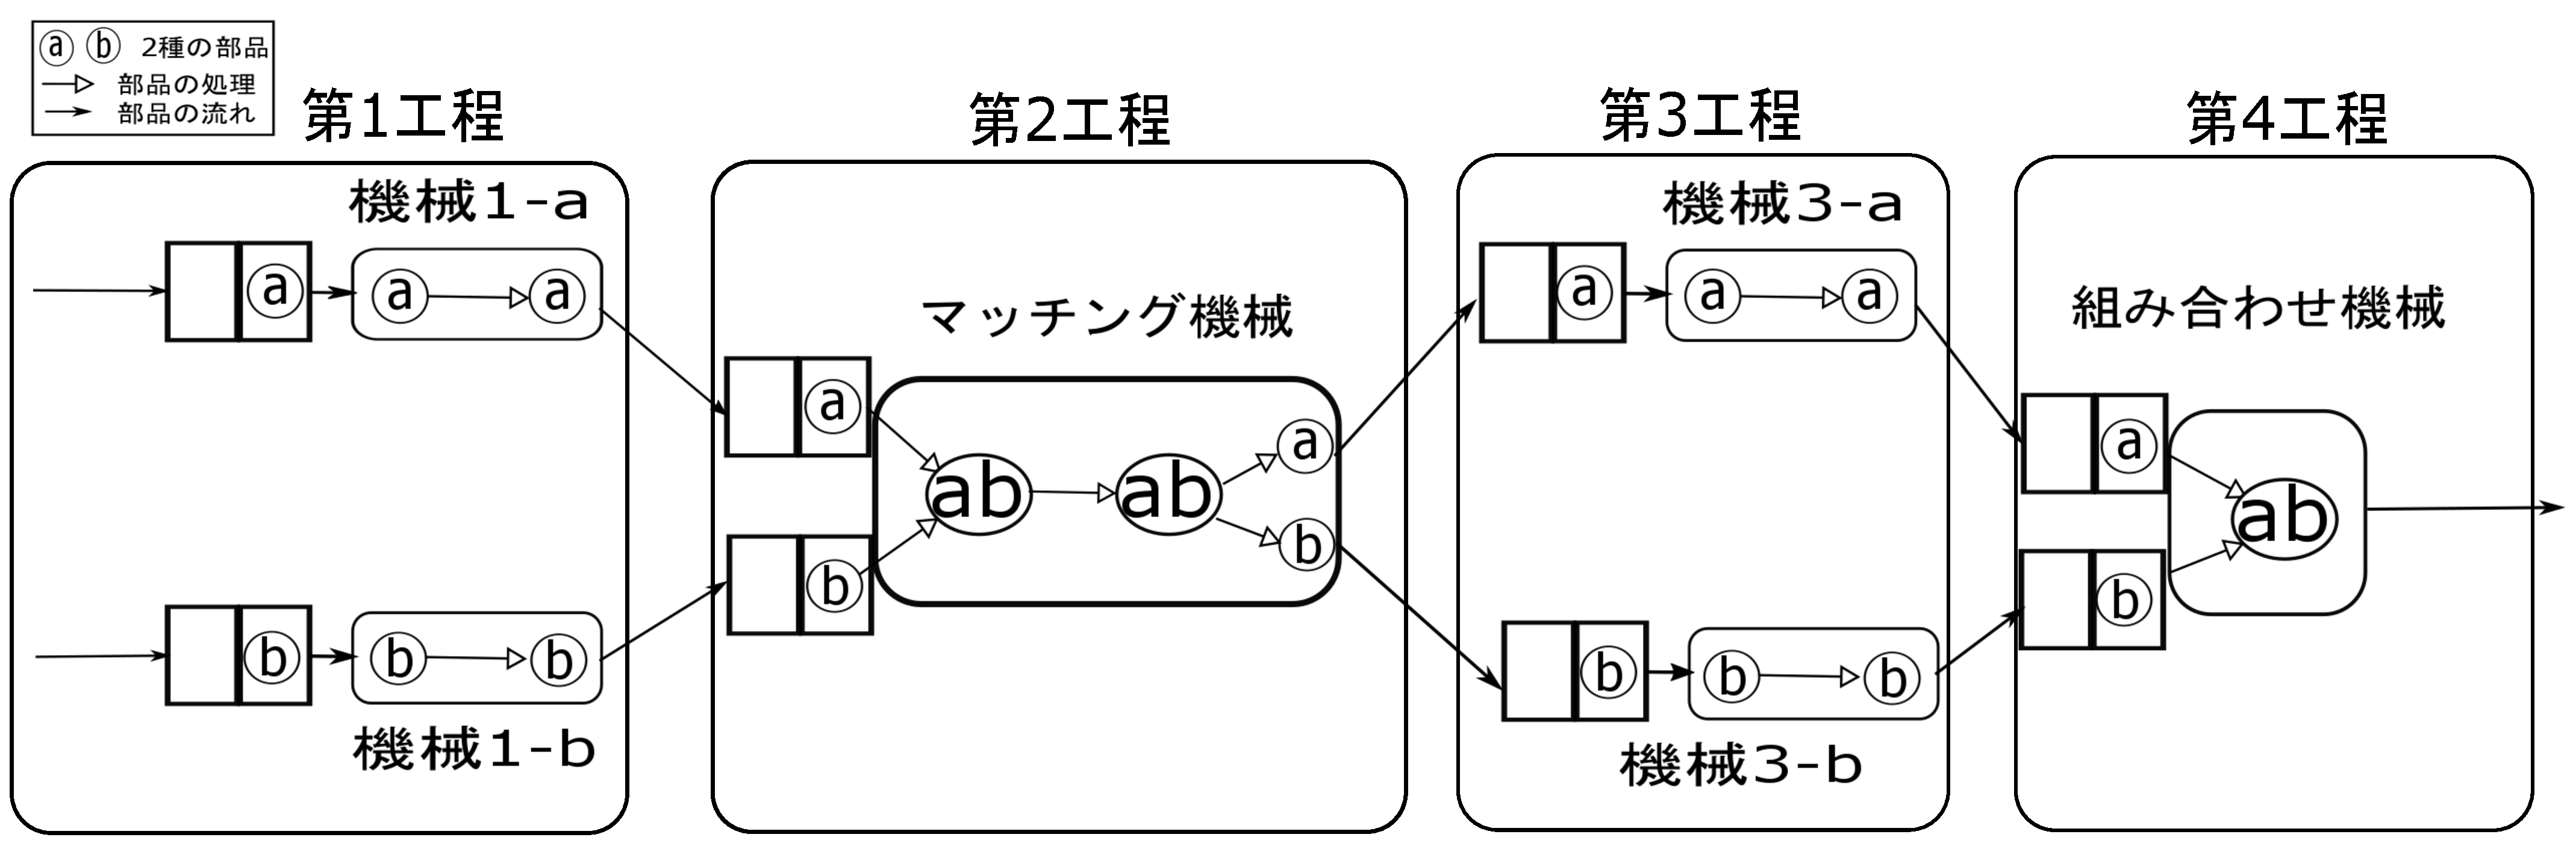
\includegraphics[clip, width=7.0cm, height = 4.0cm]{model_ver5.eps}
	\end{center}
	\caption{マッチング処理制約のある4工程FFS}
	\label{fig:model}
\end{figure}

\section{検査タイミング}
工程数が2つであるときの検査するタイミングについて考える.まず最初の条件として,不良部品をFFSから離脱させることを防ぐために,2つの部品を組み合わせシステムを離脱させる第4工程の直後では必ず検査を行うものとする.また,検査を行いシステムから離脱させる目的として不良部品によるバッファの占領を避けたいという目的があるため第2,第3,第4工程のバッファに入る直前に検査を行うのが効率がよいものと考えられる.よって工程数が2つであるとき考えられる検査のタイミングとしては,第2工程のバッファに入る前と第4工程直後,第3工程のバッファに入る前と第4工程直後,第4工程のバッファに入る前と第4工程直後の3つの場合が考えられる.また,いずれの場合も不良確率を0にすると文献 \cite{1} のモデルと一致する.

\section{数値実験}
前節までに述べた待ち行列ネットワークモデルにおける3つの検査パターンに対して性能評価を行う.性能指標としてスループットとその不良率の増加にともなう低下率を算出する.スループットは単位時間当たりに第4工程で処理されシステムから離脱する部品数で定義する.
また,低下率は以下の式によって求められる.
\begin{eqnarray*}
\mbox{低下率} &=& \left\{ (\mbox{$\beta=0$のTP})-(\mbox{$\beta$変化後のTP}) \right\}  \\ 
&\div& (\mbox{$\beta=0$のTP}) \times 100
\end{eqnarray*}
この低下率は不良率と検査工程数に影響され,本稿では検査工程数がスループットに与える影響を調べたいため,スループットの低下が不良率のみに影響される場合の低下率を調べ,その値を基準として低下率の評価を行う.
この基準となる値が表 \ref{fig:base}である.
また実験では,第1工程と第3工程のバッファの大きさを1(処理中の部品は含めない),第2工程と第4工程における各部品のバッファの大きさをそれぞれ2とした.

解析では,待ち行列ネットワークモデルを一般化確率ペトリネット(GSPN)で書き換え,GSPN解析ツールを通じて連続時間マルコフ連鎖へ変換した後に連続時間マルコフ連鎖の定常解析を行った.

表 \ref{tab:result4}, \ref{tab:result14}, \ref{tab:result24}, \ref{tab:result34} は2つの部品の到着率を$\lambda=0.7$及び$\lambda=0.3$としたときのスループット(TP)ならびに$\beta = 0$からの低下率(FR($\%$))を表している.

\begin{table}[ht]
	\centering
	\caption{不良率のみに影響される低下率}
		\begin{tabular}{| l | l |} \hline
			$\beta$ & FR \\ \hline
			0 & 0	\\ \hline
			0.02 & 11.4 \\ \hline
			0.04 & 21.7 \\ \hline
		\end{tabular}
	\label{tb:base}
\end{table}

\setcounter{table}{1}
\begin{table}[htbp]
\begin{center}
\caption{第4工程直後}
\label{tab:result4}
\begin{tabular}{cc}
\begin{minipage}{0.470\hsize}
\captionsetup{labelformat=empty,labelsep=none}
\caption{$\lambda=0.7, \mu=1$}
	\begin{tabular}{| l | l | l |} \hline
		$\beta$ & TP & FR \\ \hline
		0 	 & 0.457 & 0 \\ \hline
		0.02	 & 0.404 & 11.4 \\ \hline
		0.04	 & 0.357 & 21.7 \\ \hline
	\end{tabular}
\end{minipage}
\begin{minipage}{0.470\hsize}
\captionsetup{labelformat=empty,labelsep=none}
\caption{$\lambda=0.3, \mu=1$}
	\begin{tabular}{| l | l | l |} \hline
		$\beta$ & TP & FR \\ \hline
		0 	 & 0.254 & 0 \\ \hline
		0.02	 & 0.225 & 11.4 \\ \hline
		0.04	 & 0.198 & 21.7 \\ \hline
	\end{tabular}
\end{minipage}
\end{tabular}
\end{center}
\end{table}

\setcounter{table}{2}
\begin{table}[htbp]
\begin{center}
\caption{第1工程直後と第4工程直後}
\label{tab:result14}
\begin{tabular}{cc}
\begin{minipage}{0.470\hsize}
\captionsetup{labelformat=empty,labelsep=none}
\caption{$\lambda=0.7, \mu=1$}
	\begin{tabular}{| l | l | l |} \hline
		$\beta$ & TP & FR \\ \hline
		0 	 & 0.457 & 0 \\ \hline
		0.02	 & 0.415 & 9.17 \\ \hline
		0.04	 & 0.376 & 17.7\\ \hline
	\end{tabular}
\end{minipage}
\begin{minipage}{0.470\hsize}
\captionsetup{labelformat=empty,labelsep=none}
\caption{$\lambda=0.3, \mu=1$}
	\begin{tabular}{| l | l | l |} \hline
		$\beta$ & TP & FR \\ \hline
		0 	 & 0.254 & 0 \\ \hline
		0.02	 & 0.229 & 9.66 \\ \hline
		0.04	 & 0.206 & 18.6 \\ \hline
	\end{tabular}
\end{minipage}
\end{tabular}
\end{center}
\end{table}


\setcounter{table}{3}
\begin{table}[htbp]
\begin{center}
\caption{第2工程直後と第4工程直後}
\label{tab:result24}
\begin{tabular}{cc}
\begin{minipage}{0.470\hsize}
\captionsetup{labelformat=empty,labelsep=none}
\caption{$\lambda=0.7, \mu=1$}
	\begin{tabular}{| l | l | l |} \hline
		$\beta$ & TP & FR \\ \hline
		0 	 & 0.457 & 0 \\ \hline
		0.02	 & 0.408 & 10.7 \\ \hline
		0.04	 & 0.363 & 20.6 \\ \hline
	\end{tabular}
\end{minipage}
\begin{minipage}{0.470\hsize}
\captionsetup{labelformat=empty,labelsep=none}
\caption{$\lambda=0.3, \mu=1$}
	\begin{tabular}{| l | l | l |} \hline
		$\beta$ & TP & FR \\ \hline
		0 	 & 0.254 & 0 \\ \hline
		0.02	 & 0.225 & 11.4 \\ \hline
		0.04	 & 0.199 & 21.7 \\ \hline
	\end{tabular}
\end{minipage}
\end{tabular}
\end{center}
\end{table}

\setcounter{table}{4}
\begin{table}[htbp]
\begin{center}
\caption{第3工程直後と第4工程直後}
\label{tab:result34}
\begin{tabular}{cc}
\begin{minipage}{0.470\hsize}
\captionsetup{labelformat=empty,labelsep=none}
\caption{$\lambda=0.7, \mu=1$}
	\begin{tabular}{| l | l | l |} \hline
		$\beta$ & TP & FR \\ \hline
		0 	 & 0.457 & 0 \\ \hline
		0.02	 & 0.406 & 11.2 \\ \hline
		0.04	 & 0.359 & 21.5 \\ \hline
	\end{tabular}
\end{minipage}
\begin{minipage}{0.470\hsize}
\captionsetup{labelformat=empty,labelsep=none}
\caption{$\lambda=0.3, \mu=1$}
	\begin{tabular}{| l | l | l |} \hline
		$\beta$ & TP & FR \\ \hline
		0 	 & 0.254 & 0 \\ \hline
		0.02	 & 0.225 & 11.4 \\ \hline
		0.04	 & 0.186 & 21.7 \\ \hline
	\end{tabular}
\end{minipage}
\end{tabular}
\end{center}
\end{table}


\section{考察}
表 \ref{tab:result4}, \ref{tab:result14}, \ref{tab:result24}, \ref{tab:result34}より第1工程直後と第4工程直後において検査を行うと最もスループットの低下率が低くなるという結果が得られた.
これは不良部品が次の工程に流れていくたびに新たな不良部品を生むという条件が影響していると考えられる.
組み合わせやマッチング処理制約のある第2工程以降では,2つのラインを流れる部品のうち片方が正常であっても,もう一方が不良部品であれば正常な部品も共に廃棄されてしまうため,スループットが下がってしまう.
よって,今回のFFSにおいては不良部品の検査はマッチング処理制約の影響のない第1工程直後と第4工程直後にFFSから取り除くことが望ましいということが分かった.


\section{まとめと今後の課題}
本稿では,マッチング処理制約のある4工程FFSについて不良部品の発生が起こり得る場合について考え,その不良部品を検知するための検査を行う工程数を2つに絞りそのスループットの低下率を計算することで,工程数が2つに増えた場合どの工程において検査を行うと最もスループットが高くなるのかを調べた.

今後はシステムのバッファの数を増やしシステムの混雑度がスループットにどのように影響を与えるのかを調べていく.


\begin{thebibliography}{9}
	\bibitem{1}Hui-Yu Zhang, Qing-Xin Chen, and Ning Mao. 2016. ``System performance analysis of flexible flow shop with match processing constraint.'' International Journal of Production Research, 2016, Vol. 54, No. 20, pp.6052-6070.
\end{thebibliography}

\end{document}